%% 4. 「技術研究報告」
\documentclass[technicalreport]{./ieicej-v3.0/UTF/ieicej}
%\usepackage[dvips]{graphicx}
%\usepackage[dvipdfmx]{graphicx,xcolor}
\usepackage[T1]{fontenc}
\usepackage{lmodern}
\usepackage{textcomp}
\usepackage{latexsym}
\usepackage{amsmath}
\usepackage{amssymb, amsthm}
%\usepackage{enumitem}
\usepackage{bm}
\usepackage{type1cm}
\usepackage{ascmac} % for box
\usepackage{url}
\usepackage{algorithm}
\usepackage{algpseudocode}
%\usepackage[justification=centering]{caption}
%\usepackage{subcaption}
\usepackage[dvipdfmx]{graphicx}
\usepackage{otf}
%\usepackage{hyperref}
%\usepackage[fleqn]{amsmath}
%\usepackage{amssymb}
\makeatletter
\makeatother
\newcommand{\argmax}{\mathop{\rm arg~max}\limits}
\newcommand{\argmin}{\mathop{\rm arg~min}\limits}
\newcommand{\rme}{\mathrm{e}}



\jtitle{Friend-to-friendオーバーレイネットワークにおける\\効率的な分散ルーティング}
\jsubtitle{}
\etitle{Efficient decentralized routing in friend-to-friend overlay networks}
\esubtitle{}
\authorlist{%
 \authorentry[takahashi.akira.58s@kyoto-u.jp]{\CID{8705}橋 彰}{Akira TAKAHASHI}{Kyoto}
 \authorentry[syuji@acs.i.kyoto-u.ac.jp]{宮崎 修次}{Syuji MIYAZAKI}{Kyoto}
% \authorentry[メールアドレス]{和文著者名}{英文著者名}{所属ラベル}
}
\affiliate[Kyoto]{京都大学情報学研究科 〒606--8501 京都市左京区吉田本町}{Graduate School of Informatics, Kyoto University  Yoshida-Honmachi, Sakyo-ku, Kyoto, 606--8501, Japan}
%\affiliate[所属ラベル]{和文勤務先\\ 連絡先住所}{英文勤務先\\ 英文連絡先住所}

\begin{document}
\begin{jabstract}
%和文あらまし
Friend-to-friend (F2F)ネットワークは,各ノードが信頼のおける特定ノードとのみ通信を行う特殊なP2Pネットワークであり,Freenet等の検閲に対する耐性を重視したコミュニケーションシステムの基礎となっているが,ネットワーク上でのルーティングパフォーマンスが低いという問題点を抱えている.本研究では,次ノード選択時に隣接ノードの次数に応じた重み付けを行うというアプローチから,Freenetで用いられているルーティング手法を改良する. そしてスモールワールド性とスケールフリー性を持った信頼関係ネットワークであるWeb of Trustにおけるルーティングのシミュレーション実験を行ったところ, 今回提案するアルゴリズムが既存のFreenetにおけるルーティングアルゴリズムよりも高いパフォーマンスを発揮することを確認した. 
\end{jabstract}
\begin{jkeyword}
%和文キーワード
friend-to-friend, 分散ルーティング,複雑ネットワーク
\end{jkeyword}
\begin{eabstract}
%英文アブストラクト
Friend-to-friend (F2F) networks, connectivity-restricted P2P networks which provide censorship-resistant communication systems such as Freenet, suffer from a poor routing performance. In this paper, we improve Freenet's routing algorithm by utilizing neighbors' degree information in message forwarding. Our routing simulations in PGP Web of Trust, a real-world trust relationship network with small-world and scale-free characteristics, show that the proposed method outperforms the existing routing algorithm of Freenet.
\end{eabstract}
\begin{ekeyword}
friend-to-friend, decentralized routing, complex networks
\end{ekeyword}
\maketitle

\section{はじめに}
近年インターネットを介したコミュニケーションまたは出版は, 我々の生活において大きな位置を占めるようになってきた. それに伴いユーザーのプライバシー保護を重視したコミュニケーションツールの実装に対する需要が非常に高まっている. その要因として, 例えば近年ではEdward Snowdenによって公に明らかにされたアメリカ国家安全保障局(NSA)による大規模な大衆監視が挙げられる.

特定の企業や団体が中央集権的に管理する情報共有方式はこのような監視・漏洩のリスクが高いため, 非中央集権的な情報共有を実現するためのアプローチとしてP2P方式が頻繁に採用される.P2P方式にも様々なタイプがあるが,その中でもfriend-to-friend (F2F)\cite{bricklin2000friend}は特にピアの匿名性・プライバシー保護に重点を置いたネットワーキング方式であり,F2Fネットワークにおいて各ノードは, 信頼のおける特定ノードとのみ通信する. F2F方式では, 分散ハッシュテーブル(DHT)等とは異なり, 動的にネットワーク構造を最適化することはできず, ネットワーク構造は常に現実の信頼関係ネットワークの部分グラフに対応する. そしてネットワーク上で隣接していないノード同士がデータの送受信を行うためにはいずれかのノードが「知り合いの知り合い」を辿って他方のノードに到達するための経路を探索する必要性が生じる\cite{rogers2007disappear,roos2016analyzing}.

F2Fオーバーレイネットワークの最も代表的な実装例は, Freenet\cite{clarke2001freenet}のF2Fモード\cite{clarke2010private}であり, 基本的なプロトコルはSandbergが2006年に提案した手法\cite{sandberg2006distributed}に基づいている. Freenetでは, 信頼関係のネットワークがスモールワールド性を持つと仮定し, エッジ生成確率が以下の式(\ref{eq:kleinberg_p})のようにノード間の距離に反比例するKleibergのスモールワールドネットワークモデル\cite{kleinberg2000small}が用いられている. ただし$d(u,v)$は特定の距離空間に配置されたノード$u,v$間の距離,$Z$は正規化定数で,$Z = \displaystyle \sum_{v\in V, v\neq u}^{}d(u,v)^{-1}$である.
\begin{eqnarray}
 p(u,v)=\cfrac{1}{d(u,v)Z} \label{eq:kleinberg_p}
\end{eqnarray}
Kleinbergモデルにおいて,単純なgreedyルーティング (各ノードは隣接ノード中, 最もターゲットに近いノードを次ノードとして選択) によるホップ数期待値が$O(\log^2 n)$であることが証明されているため, FreenetにおいてはKleinbergモデルの特徴を反映するように各ノードに対して座標情報を付与することでルーティングの効率化が図られている. 

ただしFreenetには未だ様々な問題点が残っている. 第一にSandbergが提案した手法では, Kleinbergモデルの特徴を正確には反映することができないため, Freenetの実装においてはgreedyルーティングの代わりにdistance-directed depth-first search ($D^2$-$DFS$)が採用されている. しかしこの$D^2$-$DFS$アルゴリズムが特定の条件下において$O(\log^2 n)$のホップ数を達成することができないことはRoos, Strufeらにより解析的に証明された\cite{roos2016dealing}. またFreenetでは, ノードへのID割り当てアルゴリズムの一環としてノード同士がIDを交換するが, この際悪意のあるノードが虚偽のID報告を繰り返すことにより, ノードがID空間上に偏在し, 結果的にルーティングの効率性が低下するというPitch black attack\cite{evans2007routing}などの深刻な脆弱性が指摘されている. よってFreenetのF2Fモードは効率性や頑健性の面で問題点が残り, 現在もそれらを解決するための研究が続けられている.

本研究では, 以上に挙げられたFreenetの問題点のうちルーティングの効率性に着目する. 今回我々は{\c{S}}im{\c{s}}ek, Jensenらによって提案されたexpected-value navigation (EVN)\cite{simsek2008navigating}をFreenetプロトコルに適用可能な形に修正することにより, スケールフリー性を持ったF2Fネットワークにおいて既存ルーティングアルゴリズムよりも高いパフォーマンスを発揮するdegree-and-distance-directed depth-first search ($D^3$-$DFS$)を提案する. また, 先行研究のシミュレーション実験においてはルーティングの成功率が向上するように実データの恣意的な改変が施されていたが, 本研究では改変を施さない実データに対するシミュレーション実験を行うことにより, 現実のF2Fトポロジーにより近いネットワークにおけるルーティングアルゴリズムのパフォーマンス評価を行った.


 \section{Freenetプロトコル} \label{sec:freenetprotocols}
  本節ではFreenetのF2Fモード(またはDarknetモードとも呼ばれる)の概略について述べる. F2Fモードの目的はP2Pシステムにおけるノードのプライバシー保護であり, ネットワーク上の各ノードは予め信頼のおけるノードとのみ直接の通信を行う. つまり「友人と友人」(friend-to-friend)の通信のみを行うという制約を設けることによって, 信頼関係の外部にいる攻撃者によるプライバシー侵害を困難にしようというのが核心となるコンセプトである.

   この制約があるため, F2Fモードにおいては通信効率を最適化するようにネットワークトポロジー自体に変更を加えることが不可能であり, 各ノードはネットワークの全体像も把握することができない. よって, ネットワーク上で隣接していないノードどうしがデータの送受信を行うためには, Milgramのスモールワールド実験\cite{milgram67smallworld}のようにネットワーク上の中継ノードが局所的な情報のみを用いてメッセージのフォワーディングを繰り返す必要がある. 

   そこでネットワークトポロジーを変えずにルーティングを効率化するためにF2Fモードが取るアプローチが, ネットワークのID空間への「埋め込み」(embedding)である. 埋め込みとルーティングの概念図を図\ref{fig:f2f_overview}に示す.

   \begin{figure}[htb]
    \centerline{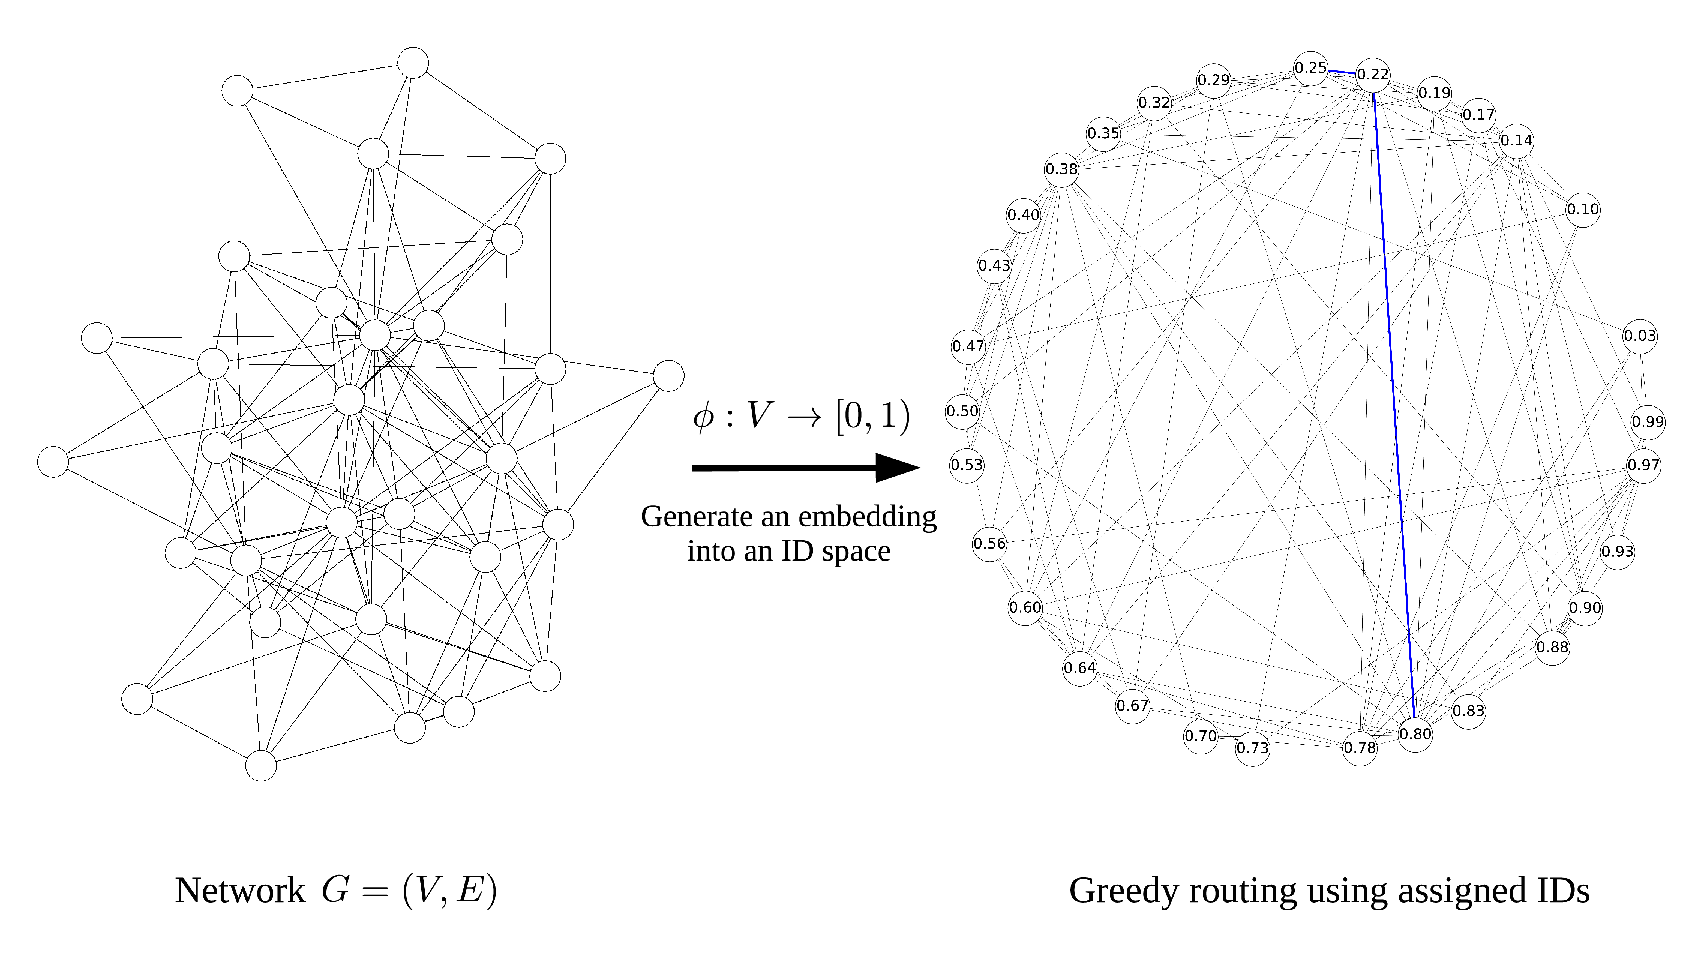
\includegraphics[width=100mm]{../fig/greedy_embedding_overview.eps}}
    \caption{F2Fネットワークにおける埋め込みとルーティングの概略}
    \label{fig:f2f_overview}
   \end{figure}

   一般的にネットワーク$G=(V,E)$の距離空間$(X,d)$への埋め込みは単射$\phi:V \to X$で定義される\cite{papadimitriou2005conjecture}. Freenetでは以下の式(\ref{eq:f2f_dist})で定義される距離関数$d$を備えた単位区間$[0,1)$が上記の$X$に対応し, ID空間(ID space)またはキー空間(key space)などと呼ばれる. 以下では空間上の一点を便宜的に``ID''または「座標」と呼ぶこととする. 図\ref{fig:f2f_overview}のようにID空間上の各点は円上の点に, 2点間の距離は円周上の距離に対応付けることができる.

   \begin{eqnarray}
    \forall x,y \in [0,1), d(x,y) = \min\{|x-y|, 1 - |x-y|]\} \label{eq:f2f_dist}
   \end{eqnarray}

   よってF2Fモードでは, 効率的な分散ルーティングが可能となるようにID空間への埋め込み$\phi$を生成することが重要となる. 埋め込みの生成はSandbergが2006年に提案した手法(以下SWAPアルゴリズムと呼ぶ)に基づいている\cite{sandberg2006distributed}. SWAPアルゴリズムは埋め込みの生成をパラメータ$\phi$の推定問題としてみなし, ID空間に埋め込まれたグラフがKleinbergのスモールワールドモデルによって生起する確率が高くなるように(つまりID空間において隣接するノード間の距離の分布が式(\ref{eq:kleinberg_p})に従うように), $\phi$をMetropolis-Hastings法によりサンプリングする.

   SWAPアルゴリズムの概略は以下の通りである.

   \begin{enumerate}
    \setcounter{enumi}{-1}
    \item
各ノードは$[0,1)$上の一様乱数を発生させ, 初期IDを得る. これを初期状態とする.

    \item
ノード$u$はID交換相手の候補$v$をネットワーク上でのランダムウォークにより選択し, ID交換リクエストを送る.

    \item
各$u,v$がそれぞれ「隣接ノードと自分の距離」「隣接ノードと相手の距離」を計算することで, 採択確率$\beta(\phi_1, \phi_2)$を得る. ただし$\phi_1$は現在の埋め込みのサンプル, $\phi_2$は候補サンプルで, $\phi_1$における$u,v$のID割り当てを入れ替えたものである.

    \item
$[0,1)$上の一様乱数を生成し乱数が$\beta(\phi_1, \phi_2)$を超えなければ, $u,v$はIDを交換, すなわち埋め込みの候補サンプル$\phi_2$を採択し, さもなくばID交換を行わない.
   \end{enumerate}

   以上の(1)から(3)までの操作を十分な回数反復することで, greedyルーティングによる平均ホップ数が短くなるようなIDの割り当てを生成することができる. Sandbergは人工的に生成したKleinbergのネットワークデータと実データに対してシミュレーション実験を行い, SWAPアルゴリズムの適用後割り当てられた座標情報が, ランダムに割り当てられた座標情報に比してgreedyルーティングの効率性を高めることを示した.

   SWAPアルゴリズムの適用は確かにgreedyルーティングの効率性を高めるようなIDの割り当てが可能であるが, 本来のKleinbergモデルと同様の$O(\log^2n)$のホップ数は保証されない. なぜなら, Kleinbergモデルでは空間上で最も距離の近いノードへのエッジ (local contact) が必ず存在しているという仮定によってgreedyルーティングの最中にターゲットまでの距離が狭義に単調減少することが保証されているが, SWAPアルゴリズムによってID空間に埋め込まれたネットワークは必ずしもこのlocal contactを持たないからである. よって単純なgreedyルーティングでは``dead-end''(自分よりもターゲットに近い隣接ノードが存在しない状態)に達してしまう. そこでFreenetでは単純なgreedyルーティングではなく,ホップ数上限付のdistance-directed depth-first search ($D^2$-$DFS$)を採用することでdead-endに対処している. $D^2$-$DFS$の次ノード選択の方法はgreedyルーティングと同様であるが,隣接ノードが全て訪問済みの場合には自らに初めてメッセージをフォワードしたノード (predecessor) にメッセージを戻すという点において異なる.

   しかしRoos, Strufeらは埋め込みの不正確さを考慮してlocal contactの存在を仮定しないKleinbergのモデルを提案し, そのようなグラフにおいて$D^2$-$DFS$がポリ対数関数(polylogarithmic)のオーダーでルーティングを終えることができないことを解析的に証明している\cite{roos2016dealing}. 

\section{問題設定}
\ref{sec:freenetprotocols}節に述べたF2Fネットワークにおける分散ルーティング効率を向上させるための大まかな方針として (i)埋め込みアルゴリズムの改良 (ii)分散ルーティングアルゴリズムの改良 の2通りを挙げることができるが,本研究では後者の方針を取る.そこで今回我々はF2Fネットワークの実データが持つスケールフリー性に着目し,次ノード選択時に隣接ノードの次数に応じた重み付けを行うルーティングアルゴリズム提案する. つまり, 今回我々が検証する仮説は「SWAPアルゴリズム適用後のF2Fネットワークにおいて, 単純なノード間距離に応じたヒューリスティックを用いる代わりに, 隣接ノードの次数とノード間距離を共に考慮したヒューリスティックスを用いることで, ルーティングのパフォーマンスを向上させることが可能である」とまとめることができる. 以下この仮説検証のために, $D^2$-$DFS$を改良したルーティングアルゴリズム, degree-and-distance-directed depth-first search ($D^3$-$DFS$)の提案と, 恣意的な前処理を施さない実データを用いたパフォーマンス評価を行っていく.

\section{提案アルゴリズム}
まず$D^3$-$DFS$において用いるヒューリスティックスを定義するために,隣接ノードの次数とノード間の類似度(homophily)を考慮したexpected-value navigation(EVN)\cite{simsek2008navigating}におけるヒューリスティックの枠組みを用いる.

   EVNの基本的なアイデアは, メッセージを持っているノード$u$の隣接ノード$v \in N(u)$からターゲットノード$t$までの経路長$l(v,t)$を考え, その期待値$E(l(v,t))$を近似的に計算し, $E(l(v,t))$を最小化するような$v$を次ノードとして選択するというものである. {\c{S}}im{\c{s}}ek, Jensenらによれば,$E(l(v,t))$の2次以降の項を無視し, さらに二項分布をポアソン分布によって近似することにより$E(l(v,t)) \approx 1- e^{k_vp(v,t)}$という簡略化が可能である. ただし$k_v$を隣接ノード$v$の次数, $p(v,t)$を$v$から$t$へのエッジが生成される確率(つまりノード間の類似度)とする.

    よってある隣接ノード$v$が$E(l(v,t))$を最小化することは, $1/k_vp(v,t)$を最小化することと同値であるからヒューリスティック関数$f(v)$を
    \begin{eqnarray}
     f(v) = \frac{1}{k_vp(v,t)}\label{eq:evn-heuristic}
    \end{eqnarray}
    と定義すれば, 「メッセージを持つノード$u$は(\ref{eq:evn-heuristic})式で定義される$f(v)$を最小化するような隣接ノード$v \in N(u)$にメッセージをフォワードする」というシンプルなルーティングアルゴリズムにより, 「隣接ノード中ターゲットまでのホップ数が最も少ないと期待されるノード」を選択することができる.

    以上に述べたEVNのヒューリスティックをFreenetプロトコルに応用するためには,Kleinbergモデルに従ってエッジが生成されたと仮定した場合の$p(v,t)$を代入すれば良い. つまりID空間$[0,1)$上にノードを持つネットワークのエッジがパラメータ$r=1$と共にKleinbergモデルに従って生成されたと仮定すると隣接ノード$v \in N(u)$がターゲットノード$t$と隣接する確率は(\ref{eq:kleinberg_p})式より, $p(v,t) = 1/d(v,t)Z$であるから, これを(\ref{eq:evn-heuristic})式に代入するとヒューリスティック関数は$f(v) = d(v,t)Z/k_v$と表すことができる.

ここで, ノードのIDがSWAPアルゴリズムに従って生成された場合, IDは$[0,1)$上に一様に分布しており, その場合正規化定数$Z$は任意のノードについて同じ値であると見なすことが出来る. よってヒューリスティック関数の大小比較のみをするのであれば$Z$の計算は省略可能である. ヒューリスティック関数を改めて$g(v)$とすれば

\begin{eqnarray}
g(v) = \frac{d(v,t)}{k_v} \label{eqn:d3dfs-heuristic}
\end{eqnarray}

よって$D^3$-$DFS$において, メッセージを持つノード$u$は(\ref{eqn:d3dfs-heuristic})式を最小にするような$v \in N(u)$にメッセージをフォワードすることが基本的な動作となる. これは通常の距離のみを用いたgreedyルーティングに次数の重み付けを付加したものと見なすことができる.

次に, $u$の全ての隣接ノードが以前にメッセージを受け取ったことがあるような状況を考える. このような場合 {\c{S}}im{\c{s}}ek, Jensenらは, 次ノードを隣接ノードの中からランダムに選択することが最適であると結論づけているが, ランダムなノード選択では同様に隣接ノードが全て訪問済みであるようなノードに何度も到達する可能性があり無駄なステップが増えることが予想されるため, $D^3$-$DFS$では$D^2$-$DFS$と同様, $u$に初めてメッセージをフォワードしたノード (predecessor) にメッセージを戻すとする.

以上$D^3$-$DFS$の動作に関する概略を述べた. 詳細なアルゴリズムは擬似コードとしてAlgorithm \ref{alg:d3dfs}に示す. 
   \begin{algorithm}[htb]
    \caption{$D^3$-$DFS(\textrm{Node } u,\textrm{ Node } p, \textrm{ ID } t,\textrm{ Set }B, \textrm{ TTL }c$)}\label{alg:d3dfs}
    \begin{algorithmic}[1]
     \State \# $u$: current message holder, $p$: previous message holder
     \State \# $t$: target node ID, $B$: set of nodes who have seen the message before
     \If {$id(u) == t$}
     \State \textrm{routing succeeded; terminate}
     \EndIf
     \If {$c$ == 0}
     \State \textrm{routing failed; terminate}
     \EndIf
     \If {$u.predecessor$ == null}
     \State $u.predecessor \gets p$
     \EndIf
     \State $S \gets \{v \in N(u) |  v \notin B \}$
     \If {$S == \o$}
     \State $B \gets B \cup \{u\}$
     \State $next \gets u.predecessor$
     \Else
     \State $next \gets \argmin_{v \in S} d(u, v)/k_v$
     \State $B \gets B \cup \{ next\}$
     \EndIf
     \If {$next == \textrm{null}$}
     \State \textrm{routing failed; terminate}
     \Else
     \State $D^3$-$DFS(next, u, t, B, c-1)$
     \EndIf
    \end{algorithmic}
   \end{algorithm}
   
最後に$D^3$-$DFS$において各ノードが利用可能な情報をまとめると以下のようになる.

   \begin{enumerate}
    \item 自分と隣接ノードのID

    \item ターゲットのID

    \item 隣接ノードの次数
   \end{enumerate}

上記の(1),(2)はFreenetにおける$D^2$-$DFS$が利用する情報と同様であるが, (3)は新たに追加された情報である. 実際のF2Fネットワークにおける実装においては, 各ノードが互いに現在の接続ノード数に関する情報を隣接ノードと共有し合う状況ということになる.隣接ノードの単なる次数情報はグラフ全体のトポロジーを明らかにするものではなく, 信頼するノード以外に対してアイデンティティを明かすことにもなりえないため, $D^3$-$DFS$はプライバシーコントロールやセキュリティ面を重視するFreenetなどのF2Fネットワークに十分適用可能であると考えられる.

 \section{評価} \label{sec:evaluation}
  \subsection{シミュレーション手法}
  $D^3$-$DFS$のパフォーマンス評価を行うために\ref{sec:wot}節で述べる実データに対するシミュレーション実験を行った. 実験の基本的な流れは先行研究と同様 (i)埋め込みの生成 (ii)ID空間における分散ルーティングの実行 という2つのステップから成る.

  (i)においては\ref{sec:freenetprotocols}で述べたSandbergの埋め込みアルゴリズムを適用し, 各ノードに対するIDの割り当てを行った. ただし, \cite{sandberg2006distributed}に従いMetropolis-Hastingsアルゴリズムの反復を$6000|V|$回, \cite{roos2016analyzing}に従いSWAPアルゴリズムにおけるランダムウォークの試行回数を10と設定した.

  ID割り当ての終了後, (ii)においては全てのノードを出発点として, 各ノードにつき5つのターゲットノードをランダムに選びルーティングのシミュレーションを行った. ただし\cite{sandberg2006distributed}や\cite{schiller2011attack}に従いルーティングの寿命(time-to-live)$TTL\approx \log^2|V|$とし, 1ホップをカウントするごとに$TTL$を1減らし, $TTL=0$となった時点でルーティングを失敗とみなした\footnote{実際のFreenetの実装においてはリクエストの発信者やデータの保持者の匿名性を保つために, $TTL$が最大値または1の場合は$TTL$の減少が確率的に行われる. 詳細は\cite{roos2016analyzing}等を参照.}.なお以下ではルーティングの「成功率」を ($TTL$が0になる前にターゲットの探索が完了したルーティング試行の数)/(全ルーティング試行の数) として定義する.

  以上の条件下で$5|V|$回$D^3$-$DFS$のルーティングシミュレーションを行い, ルーティングの成功率, 成功したルーティング試行の平均ホップ数を集計した. また比較のために$D^2$-$DFS$アルゴリズムに対しても同様の実験を行った.

  また成功率の異なるルーティングアルゴリズム間で平均ホップ数の大小を比較するのは不適切であるため, $TTL$を長めに(恣意的ではあるが本研究では$500$とする)設定してルーティング実験を同様に$5|V|$回行った場合の「各ホップ数以下で成功したルーティング試行の割合」を集計した.

  \subsection{使用データ} \label{sec:wot}
  F2Fネットワークに関わる先行研究の多くは埋め込みやルーティングアルゴリズムのパフォーマンス評価のため, 実世界のソーシャルネットワークデータを使用している. なぜならFreenetのような実際にデプロイされているF2Fネットワークはその性質上ネットワーク全体のトポロジーを把握することが不可能であり, 代わりに信頼関係を表すソーシャルネットワークデータがF2Fネットワークトポロジーを近似するものと考えられるからである. 本研究もそれに倣いF2Fネットワークの実データとして, 2016年12月11日時点におけるPretty Good Privacy (PGP)のWeb of Trust (WoT)を用いた. PGPは暗号化プログラムであり, WoTはPGP公開鍵の信頼性を非中央集権的な方法で担保するための仕組みである\cite{zimmermann1995official}. WoTの形成するネットワークは現実世界における人同士の信頼関係ネットワークの部分グラフであり, 公開鍵の所有者はノードに, 公開鍵に対するデジタル署名がエッジに対応する. 

  WoTは本来有向グラフであるが, 先行研究に従い「公開鍵の所有者間で相互にデジタル署名が行われている」ことを「ノード間に信頼がある」と定義する. よって元のネットワークデータから単方向の署名に対応するエッジを削除したものからgiant component (最もノード数の多い連結部分グラフ) を抽出することによって得られたグラフを信頼関係ネットワーク$G=(V,E)$とする. ここで$G$は無向グラフと見なすことができる. 
  \begin{table}[htb]
   \begin{center}  
    \begin{tabular}{|c|c|} \hline
    総ノード数 $|V|$ & 48983 \\ \hline
    総エッジ数 $|E|$ & 183840 \\ \hline
    平均最短経路長 & 6.60 \\ \hline
    直径 & 35 \\ \hline
    平均次数 &  7.51 \\ \hline
    最大次数 & 885 \\ \hline
    クラスタリング係数 & 0.31\\ \hline
    スケーリング指数 & 1.92 \\ \hline
    \end{tabular}
   \end{center}
   \caption{2016年12月11日時点におけるWeb of Trustの基本情報 \\ 使用データセット: \url{https://wot.siccegge.de/download/2016-12-11.wot}}
   \label{table:wot_info}
  \end{table}
    \begin{figure}[htb]
     \begin{center}
      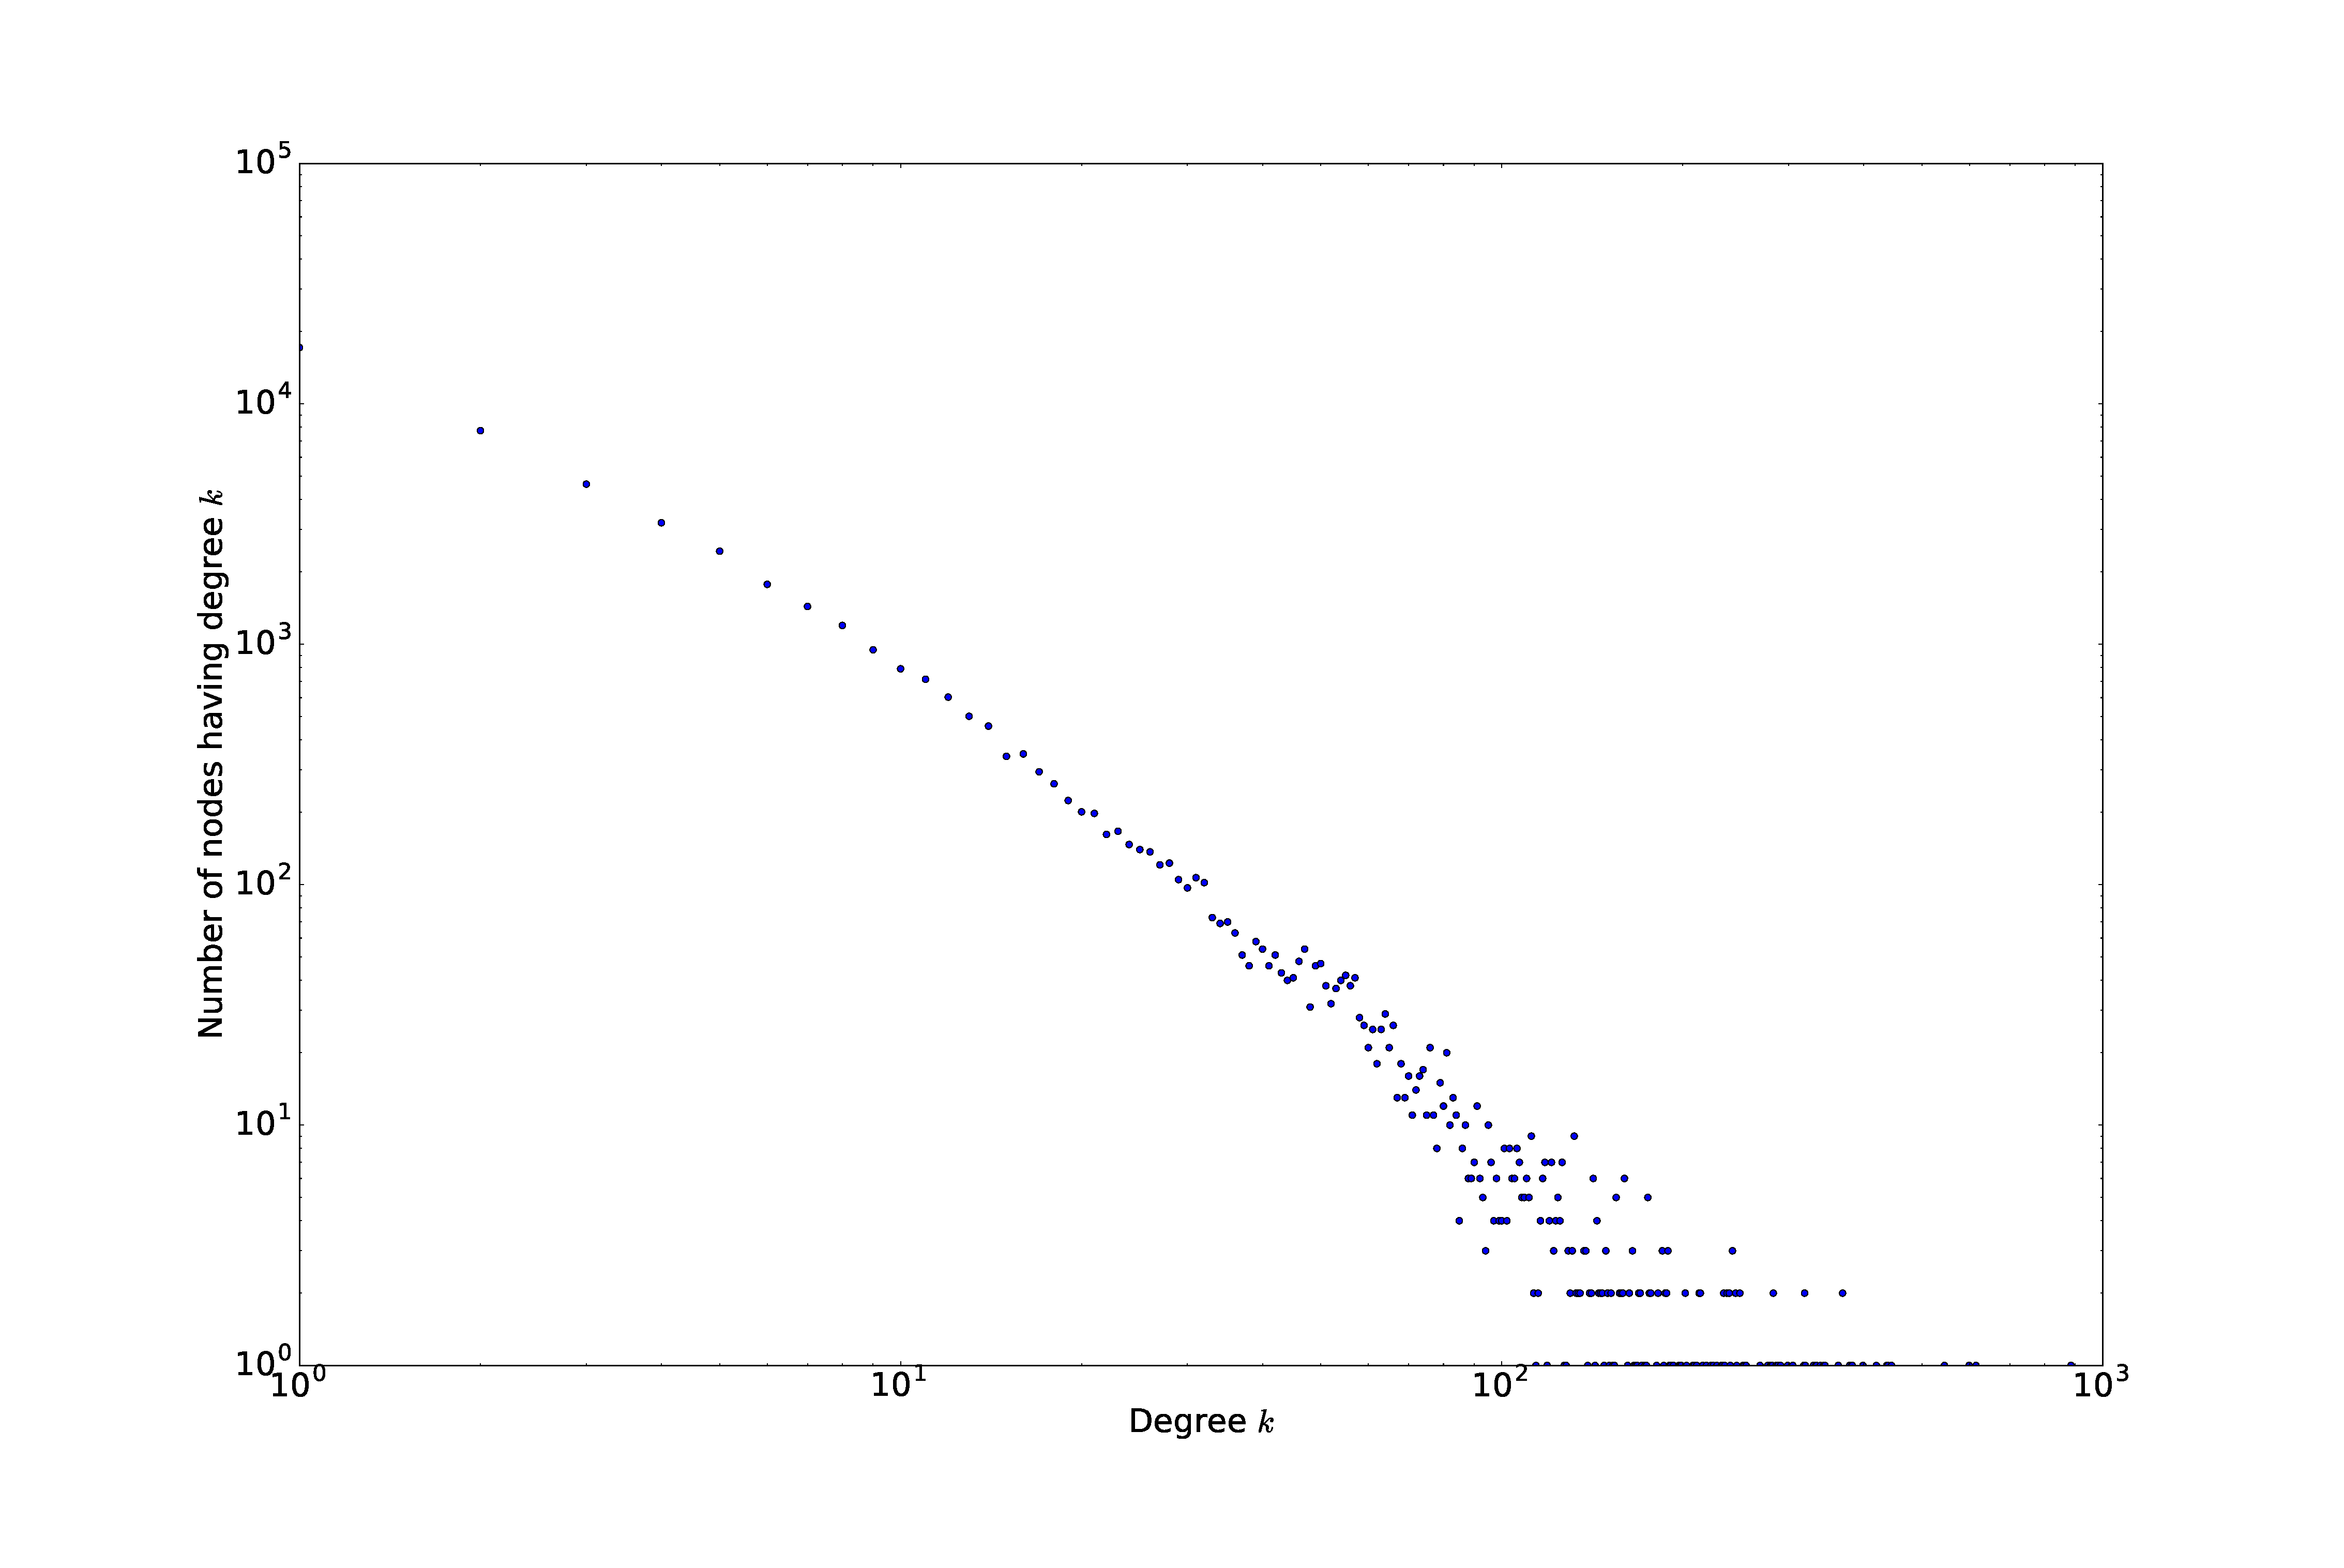
\includegraphics[width=80mm]{../fig/wot_degree_distribution.eps}
     \end{center}
     \caption{Web of Trustネットワークの次数分布}

     \label{fig:wot_dd}
    \end{figure}

  WoT $G$の解析の結果判明したネットワークの特徴を表\ref{table:wot_info}に示す. なお平均最短経路長はDijkstra法により, スケーリング指数については最小二乗法により求めた. 表\ref{table:wot_info}とWoTの次数分布をプロットした図\ref{fig:wot_dd}に見られるように, 高いクラスタリング係数, 小さな平均最短経路長, べき則に従う次数分布等, 典型的なスモールワールドネットワークかつスケールフリーネットワークの特徴が確認できる. 

 WoTをシミュレーション用実データとして用いている\cite{sandberg2006distributed}や\cite{clarke2010private}では以上に述べたのと同様の前処理の後さらにネットワークの局所的な部分グラフを取り出したり, 低次数ノードを削除するなどの操作を加えた後シミュレーションを行っているが, 本研究では現実のF2Fネットワークトポロジーにおけるルーティングのパフォーマンスをより正確に評価するために, そういった意図的な操作は施さずにシミュレーションを行う. 以下では無向グラフとみなせる部分グラフを抽出する最低限の前処理が施されたのみで, 意図的な操作が加えられていないデータを便宜的に「未処理のネットワーク」と呼ぶこととする.

なお今回行ったシミュレーションに関わる全てのソースコードはGitHubレポジトリ(\url{https://github.com/akiratk0355/navigable-network-analysis})にて閲覧可能である.

  \subsection{シミュレーション結果}
   まずWoTネットワークにSWAPアルゴリズムを適用し,ID空間に埋め込んだ様子を図\ref{fig:wot_emb}に示す. Kleinbergモデルによって生成されたグラフと同様に「距離が近いノードどうしほどエッジを持ちやすい」という特徴が現れており, Kleinbergモデルの性質が「復元」されたのが視覚的にも確認出来る.

   またlocal contactの存在率を$p_{\rm{local}}=$(ID空間上で最も近距離にいるノード同士を接続するエッジの本数)$/|V|$と定義し,初期状態とSWAPアルゴリズム適用後のグラフについてそれぞれ$p_{\rm{local}}$を算出した.その結果ランダムにIDを割り当てた初期状態において$p_{\rm{local}}=0.0002$だったのに対し,図\ref{fig:wot_emb}では$p_{\rm{local}} = 0.23$と大幅に改善してはいるものの,1.0からは程遠いため, 埋め込み後のネットワークにおける単純なgreedyルーティングの効率性が担保されないことが, この時点ですでに予測される.

   \begin{figure}[htb]
    \includegraphics[width=80mm]{../fig/wot_emb_sandberg_thesis.png}
    \caption{SWAPアルゴリズムによりID空間$[0,1)$に埋め込まれたWeb of Trustネットワーク}
    \label{fig:wot_emb}
   \end{figure}

   次に図\ref{fig:wot_emb}のネットワークに対するルーティングシミュレーションを行った結果を表\ref{table:succ_hops_full}と図\ref{fig:simple_cml_noclip}に示す.  シミュレーションの結果$D^3$-$DFS$は$D^2$-$DFS$を15\%以上成功率で上回り, にも関わらず平均ホップ数を20以上短縮するという大幅なパフォーマンスの改善を見せた.また図\ref{fig:simple_cml_noclip}の通り,$TTL$を500以下のどのような値に設定したとしても,$D^3$-$DFS$が既存アルゴリズムよりも高い成功率を実現することが可能であることを確認できた.

  \begin{table}[htb]
   \begin{center}  
    \begin{tabular}{|c|c|c|} \hline
    & $D^2$-$DFS$ & $D^3$-$DFS$ \\ \hline
    成功率 & 0.23 & 0.38\\ \hline
    平均ホップ数 & 87 & 64\\ \hline
    \end{tabular}
   \end{center}
   \caption{ID割り当て後のWeb of Trustネットワークにおける各ルーティングアルゴリズムの成功率と平均ホップ数}
   \label{table:succ_hops_full}
  \end{table}
  \begin{figure}[htb]
   \centerline{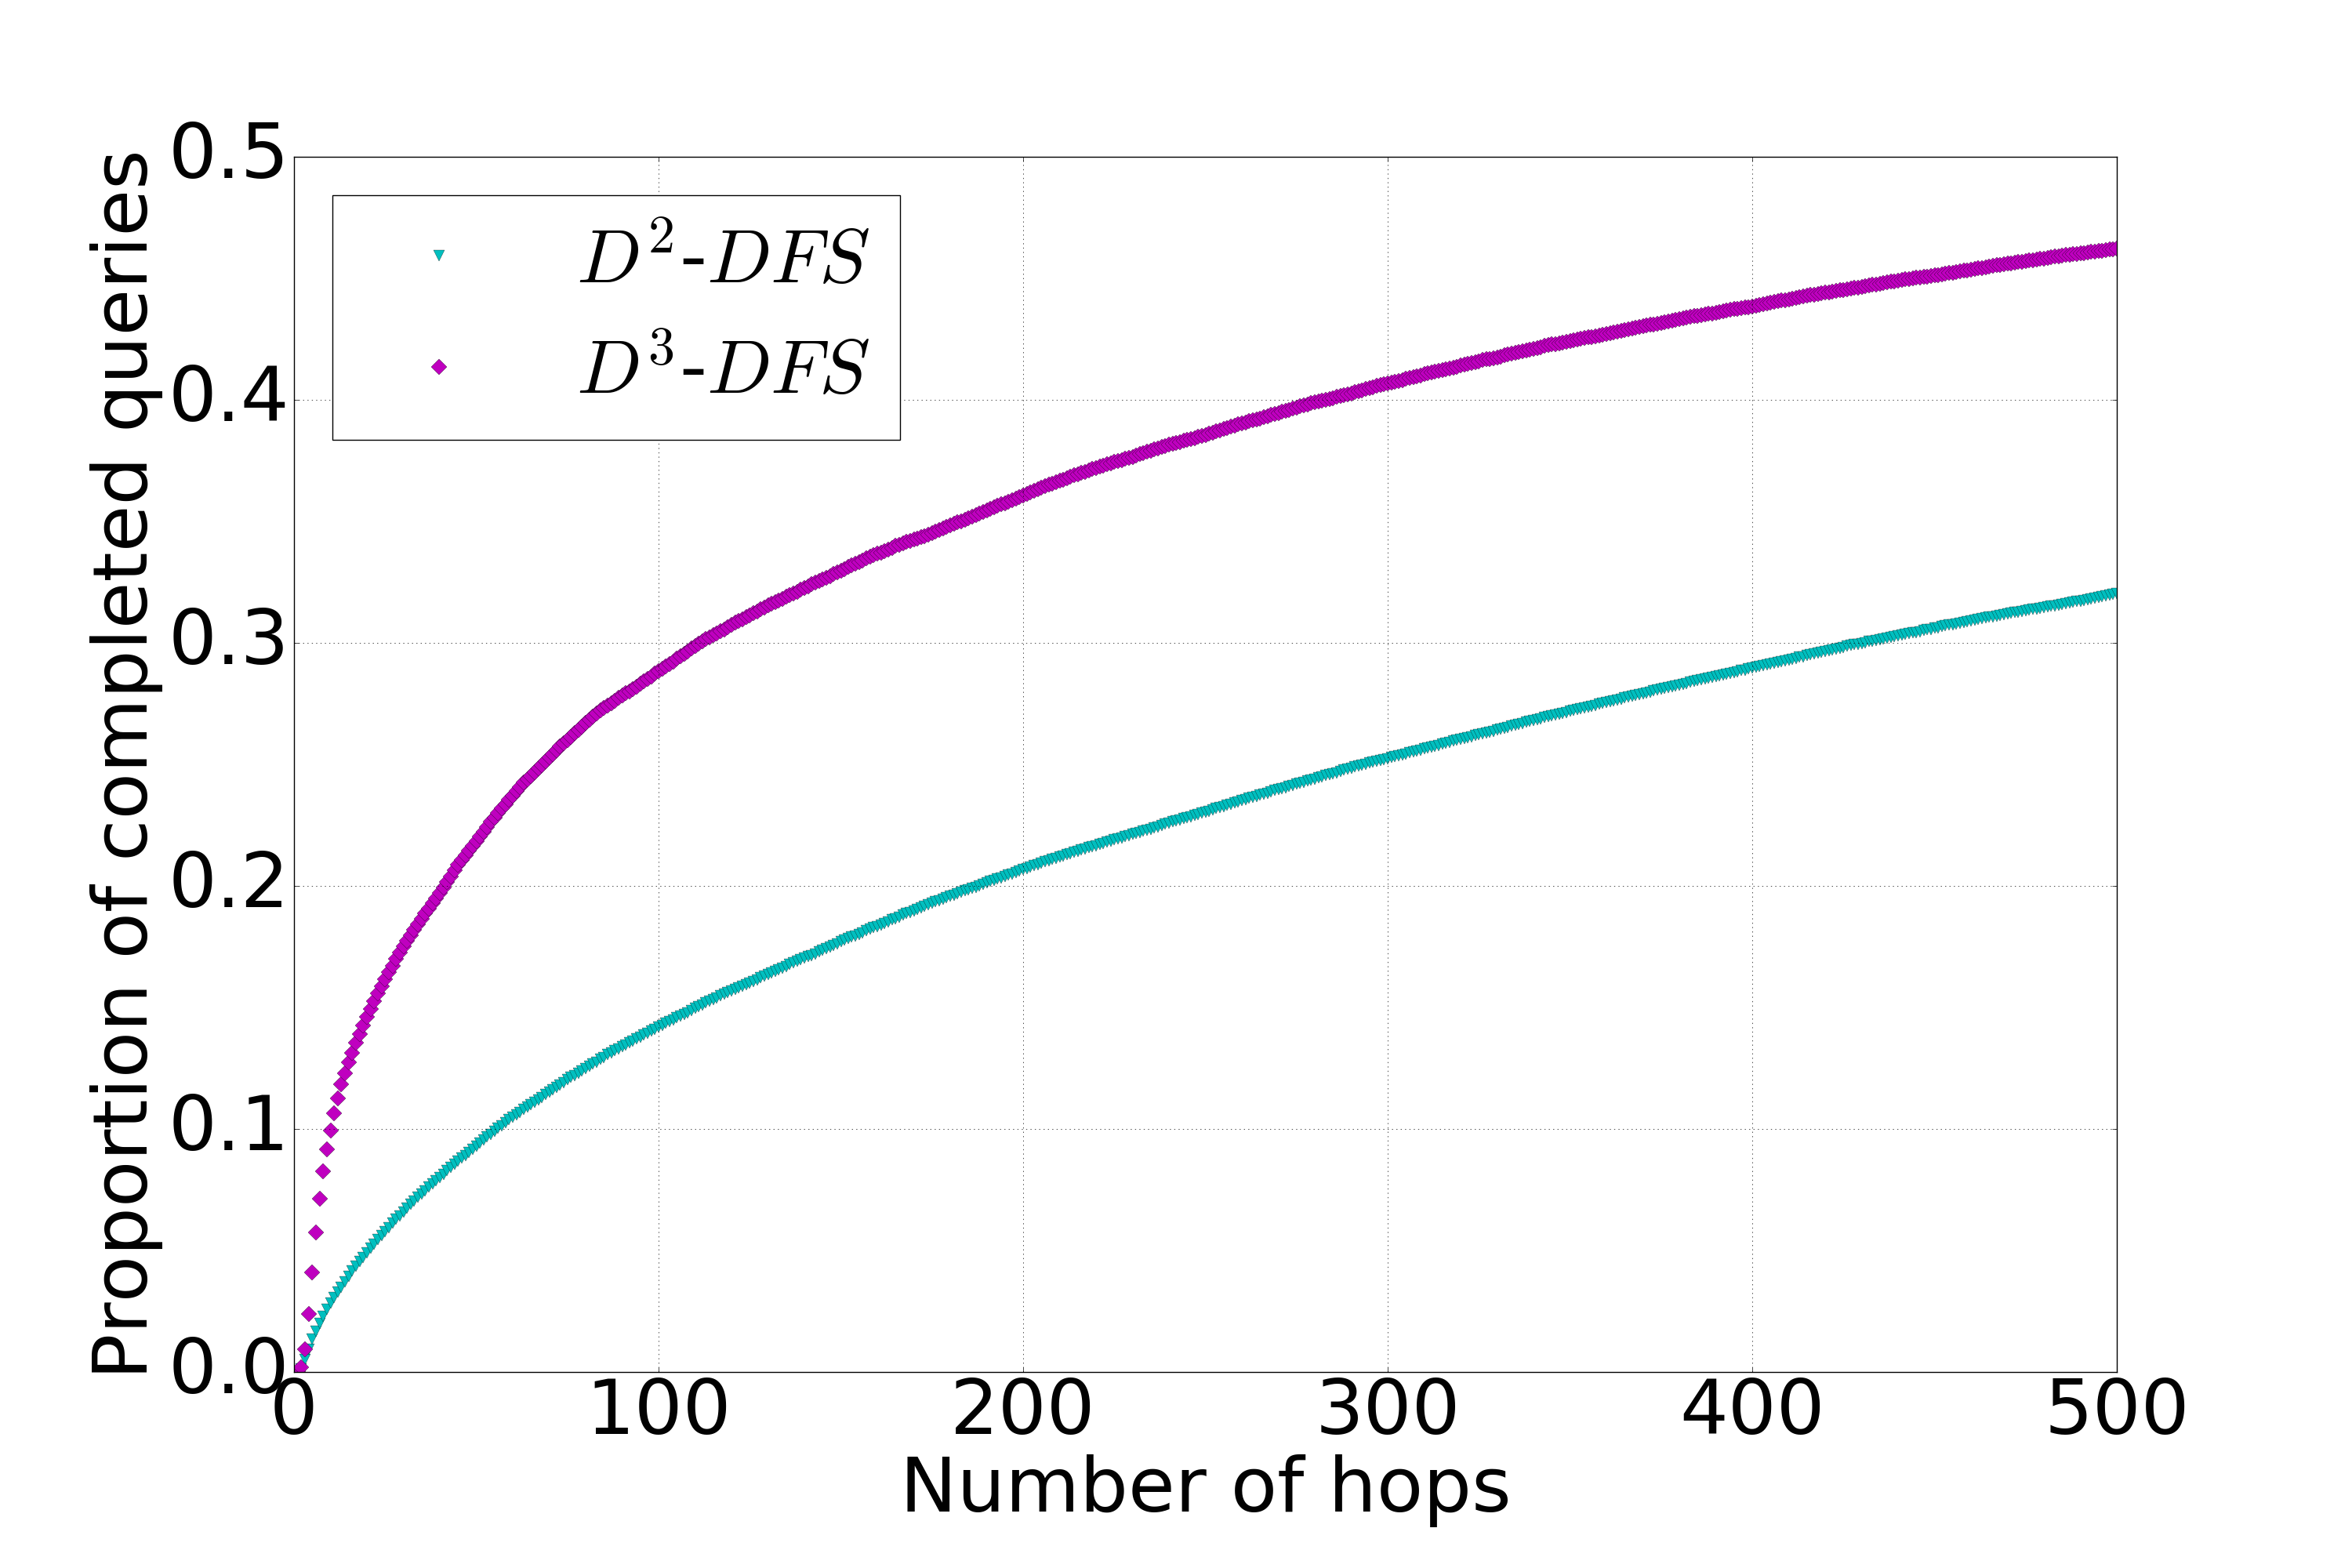
\includegraphics[width=80mm]{../fig/simple_cml_noclip.png}}
   \caption{ID割り当て後のWeb of Trustネットワークにおける各ホップ数以下で成功したルーティング試行の割合}
    \label{fig:simple_cml_noclip}
  \end{figure}

\section{まとめと今後の課題}
本研究ではF2Fネットワークにおける分散ルーティングの手法として主にFreenetのプロトコルを概観した. そしてSandbergの埋め込み生成アルゴリズムをWeb of Trustネットワークデータに適用し, ルーティングシミュレーションを行うことにより, ピュアなF2Fネットワークトポロジーにおける従来のルーティングアルゴリズムのパフォーマンスを実証的に確認した.

その上で分散ルーティングの効率性を向上させるために $D^2$-$DFS$に隣接ノードの次数を考慮したヒューリスティックを加えた$D^3$-$DFS$を提案し, そのパフォーマンス評価を行った. その結果$D^3$-$DFS$が$D^2$-$DFS$を成功率や平均ホップ数の面で凌ぐことが確認できたため, Freenet等の実際にデプロイされているF2Fネットワークの実装に活用できる可能性が大いにある. 

しかし$D^3$-$DFS$といえども今回の実験では成功率が40\%弱であり, それ自体決して高い値とは言えない. また表\ref{table:wot_info}の通り今回用いたWeb of Trustネットワークにおける本来の平均最短経路長が6.60であるの対し, $D^3$-$DFS$の平均ホップ数は依然60以上と最適値には程遠い. P2Pネットワークへの応用を考えた場合, ノード間の通信効率を保証するためにも他ノード到達の成功率を高く保ちホップ数を抑えることは非常に重要であるため, これらのパフォーマンス指標をさらに改善させることが, ピュアなF2Fネットワークを実用的なレベルにまで押し上げるための今後の課題である. 例えば今回次ノード選択のヒューリスティックにEVNを用いたが, 更に高いパフォーマンスを発揮するヒューリスティックを今後模索すべきであろう. また今回埋め込みアルゴリズムは先行研究のSWAPをそのまま用いたが, greedyルーティングが効率的となる様々な埋め込みのアルゴリズムが他にも提案されている. よって他の埋め込みアルゴリズムを適用した後のネットワークにおいて$D^3$-$DFS$が更に良いパフォーマンスを発揮できるか否か検証するべきだろう.
\bibliographystyle{./ieicej-v3.0/UTF/sieicej}
\bibliography{refs}
%\begin{thebibliography}{99}% 文献数が10未満の時 {9}
 %\end{thebibliography}

\end{document}
